\documentclass[tikz,convert={outfile=icon.svg}]{standalone}

\definecolor{myblue}{RGB}{0, 153, 255}
\definecolor{mybluedark}{RGB}{0, 51, 255}
\definecolor{mygray}{RGB}{153, 153, 136}
\definecolor{mygreen}{RGB}{0, 153, 51}
\definecolor{mypink}{RGB}{204, 51, 255}
\definecolor{mypurple}{RGB}{102, 0, 204}
\definecolor{myred}{RGB}{204, 0, 0}
\definecolor{myyellow}{RGB}{255, 204, 0}

\usetikzlibrary{calc, positioning, shapes}

\begin{document}
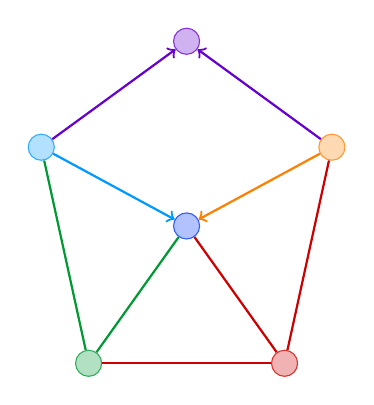
\begin{tikzpicture}
	\node[circle, draw = mybluedark!80, fill = mybluedark!30] (1) {};
	\node[circle, draw = mygreen!80, fill = mygreen!30, below left = 1.5cm and 1cm of 1] (2) {};
	\node[circle, draw = myred!80, fill = myred!30, below right = 1.5cm and 1cm of 1] (3) {};
	\node[circle, draw = orange!80, fill = orange!30, right = 1.5cm of 1, yshift = +1cm] (4) {};
	\node[circle, draw = mypurple!80, fill = mypurple!30, above = 2cm of 1] (5) {};
	\node[circle, draw = myblue!80, fill = myblue!30, left = 1.5cm of 1, yshift = +1cm] (6) {};

	\draw[thick]
		(1) edge[mygreen] (2)
		(1) edge[myred] (3)
		(1) edge[<-, orange] (4)
		(1) edge[<-, myblue] (6)
		(2) edge[myred] (3)
		(3) edge[myred] (4)
		(4) edge[->, mypurple] (5)
		(5) edge[<-, mypurple] (6)
		(6) edge[mygreen] (2);
\end{tikzpicture}
\end{document}